\section{Convex Optimization Problem}

\begin{definition}[Convex Set]
	A set $\mathcal{C}$ is convex if and only if
	$\theta x + (1-\theta)y \in \mathcal{C}$,
	$\forall\ x,y \in \mathcal{C}$,
	$\forall\ \theta \in [0,1]$
\end{definition}

(hyperplane $\parallel$ half-space)
$\{x \in \mathbb{R}^n \mid a\T x(=\parallel\le)b\}$

polyhedra $\{x\in\mathbb{R}^n\mid A^{q\times n}x\preceq b^{q\times1},C^{r\times n}x=d^{r\times1}\}$

% $A \in \mathbb{R}^{q\times n},\ C \in \mathbb{R}^{r\times n},\ b \in \mathbb{R}^{q},\ d\in \mathbb{R}^{r}$

\subsection{Operations that preserve convexity (sets)}

\textbf{Intersection}
$\mathcal{C}_1, \mathcal{C}_2$ cv
$\Rightarrow \mathcal{C}_1 \cap \mathcal{C}_2$ convex \textbf{(cv)}

\textbf{Image under affine map}
$\mathcal{C} \subseteq  \mathbb{R}^{n}$ cv
$\Rightarrow \{Ax+b \mid x \in \mathcal{C} \}$ cv

\textbf{Inverse IoaM}
$\mathcal{C} \subseteq  \mathbb{R}^{m}$ cv
$\Rightarrow \{x\in\mathbb{R}^{n} \mid  Ax+b\in\mathcal{C}\}$ cv

\subsection{Separating Hyperplane Theorem}

\begin{theorem}
	$\mathcal{C} \subseteq \mathbb{R}^{n}$ non-empty closed \textbf{(cl)} convex set, $y \notin \mathcal{C}$
	$\rightarrow \exists\ a \ne 0, b \in \mathbb{R}$
	s.t. $a\T x + b < a\T y + b,
		\forall x \in \mathcal{C}$
\end{theorem}

\begin{corollary}
	$\mathcal{C}_\text{cl,cv}$: intersection of cl half-spaces that contain $\mathcal{C}$
\end{corollary}

\subsection{Support function}

\textbf{Idea} represent any cl,cv set by its supporting hyperplanes
\[\begin{aligned}
		\vspace{-2mm}
		\sigma_\mathcal{C}(a) & = \sup_{x \in \mathcal{C}}a\T x
		\quad\text{if known, one can construct}                                                                                                        \\
		\vspace{-2mm}
		\mathcal{C}           & = \bigcap_{a \in \mathbb{R}^n} \{x \in \mathbb{R}^n \mid a\T x - \sigma_c(a) \leq 0\}                                  \\
		\vspace{-2mm}
		                      & = \{x \in \mathbb{R}^n \mid \underset{a \in \mathbb{R}^{n}}{\operatorname{sup}}\ a\T x - \sigma_\mathcal{C}(a) \le 0\}
		\vspace{-2mm}
	\end{aligned}\]

\begin{definition}
	$f:\mathbb{R}^n \rightarrow \mathbb{R}$ cv
	$\Leftrightarrow$
	epigraph of $f$ is cv set
	$$\operatorname{epi}(f):=\{(x,t)\in \mathbb{R}^{n+1} | f(x)\le t\}$$
\end{definition}

$\rightarrow$ this provides a link between convex sets and functions

\subsection{Operations that preserve convexity (functions)}

- the point wise maximum of convex functions is convex

- the sum of convex functions is convex

- $f(Ax+b)$ is convex if $f$ is convex

\textbf{Check Convexity} $f$ is convex if it is
composition of simple convex function
with convexity preserving operations
or if

$f: \mathbb{R}^n \rightarrow \mathbb{R}$ twice differentiable,
$\partial^2f/\partial x^2 \succeq 0\ \forall\ x \in \mathbb{R}^{n}$

$g: \mathbb{R} \rightarrow \mathbb{R}$ with $g(t)=f(x+tv)$
convex in $t\ \forall\ x,v \in \mathbb{R}^{n}$
$\rightarrow f$ convex (restriction to a line)

\textbf{Extended real numbers} $\bar{\mathbb{R}} = \mathbb{R} \cup \{+\infty, -\infty\}$

\textbf{Indicator function}
$\psi_\mathcal{C}(x) := \begin{cases} +\infty &\text{if } x \notin\mathcal{C} \ge 0 \\ 0 &\text{if } x \in\mathcal{C} \end{cases}$

$\rightarrow$ this provides another link between convex sets and functions

We can write
$\min_{x \in \mathcal{C}}f(x)$ as
$\min_{x \in \mathbb{R}^{n}}f(x) + \psi_\mathcal{C}(x)$

\begin{definition}[3]
	$f: \mathbb{R}^{n}\rightarrow\bar{\mathbb{R}}$ is called proper
	if $f$ is bounded below and
	if $\exists\ x \in \mathbb{R}^{n}$ s.t. $f(x)<\infty$
\end{definition}

\begin{definition}[Legendre Transformation]
	The \textbf{conjugate function} of $f: \mathbb{R}^{n}\rightarrow\bar{\mathbb{R}}$  is defined as
	\textcolor{hltext}{\hl{ $f^*(y)=\sup_{x \in \mathbb{R}^{n}}y^T x-f(x)$ }}
\end{definition}

\textbf{Concave}
$\nabla_x^2 f^* \prec0$
$\Rightarrow$
maximizer of sup satisfies
$\nabla_x f^* = 0$

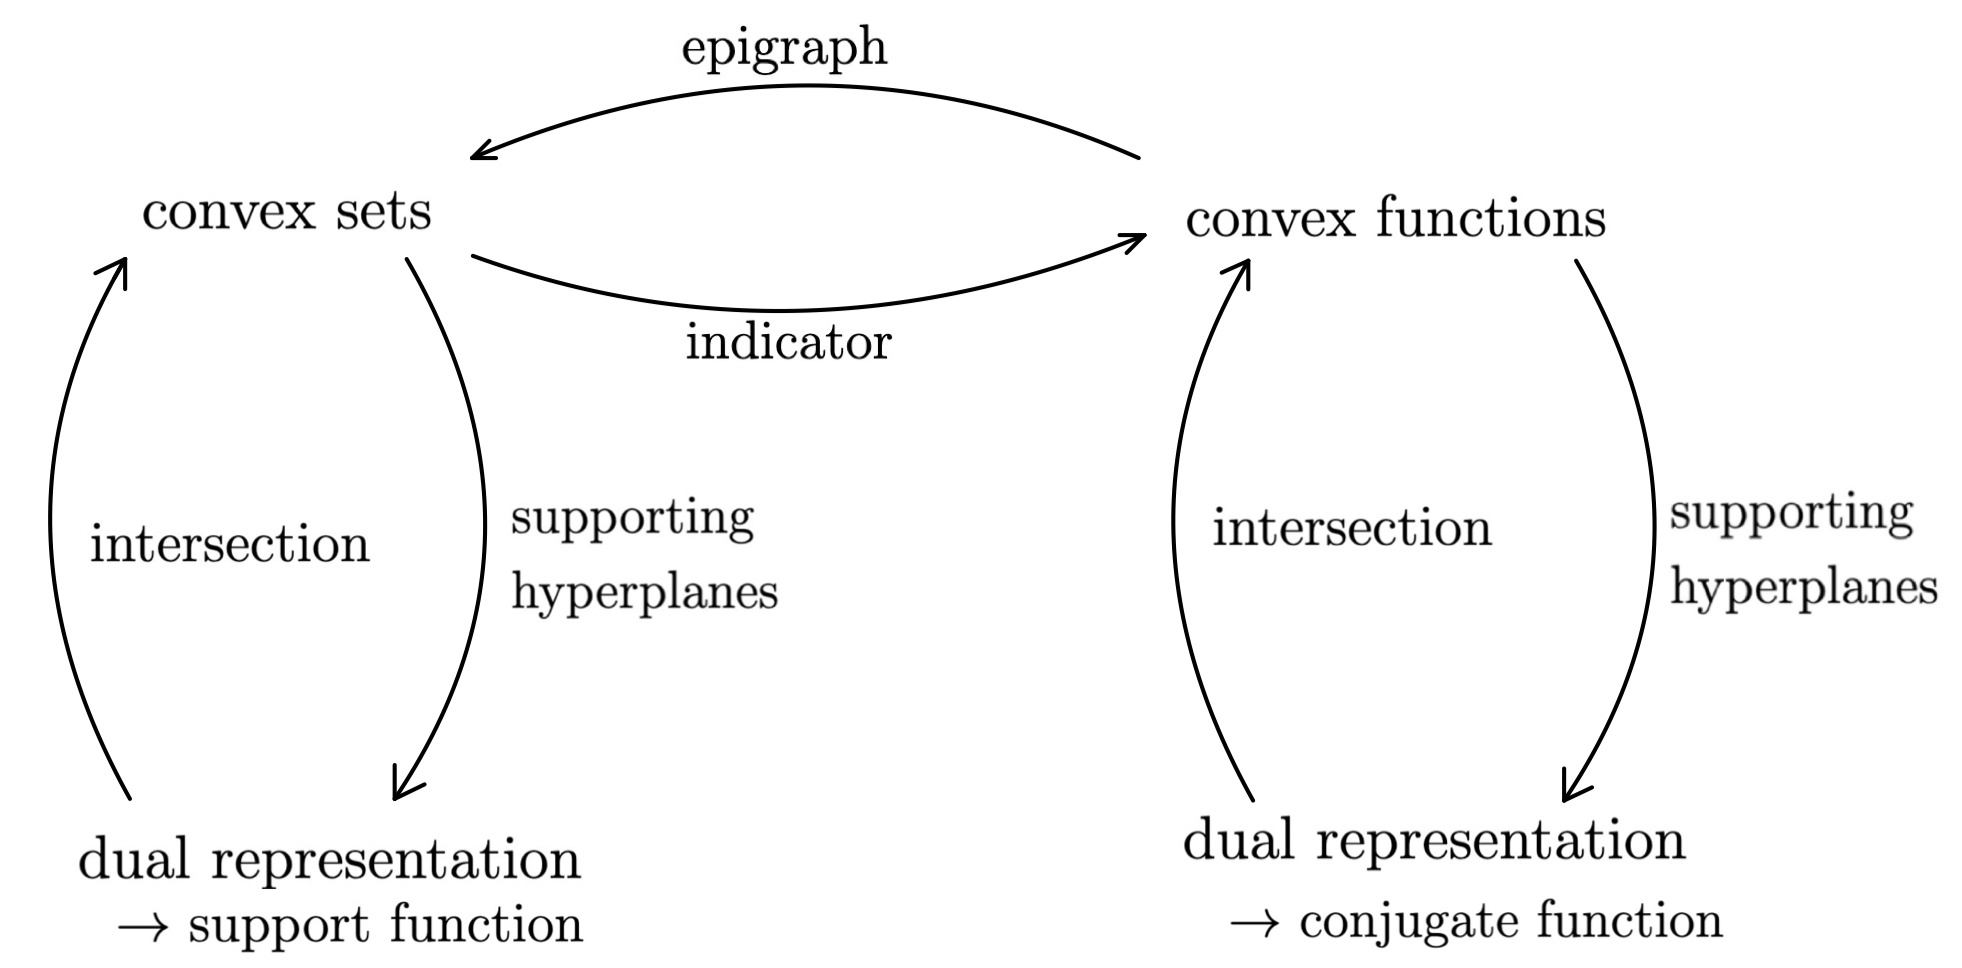
\includegraphics[width=\columnwidth]{images/summary_set_functions.png}

\begin{theorem}[Conjugate of Conjugate]
	$f:\mathbb{R}^{n}\rightarrow\bar{\mathbb{R}}$

	(i) $f$ proper, cv, epi$(f)$ closed
	$\Rightarrow f^{**}=f$

	(ii) $f(x)\ge f^{**}(x), \forall x\in\mathbb{R}^{n}$
\end{theorem}
